\[
\bar{\mathbf{x}}=\begin{bmatrix}0.564\\0.603\end{bmatrix},\qquad \mathbf{S}=\begin{bmatrix}0.014\,4 & 0.011\,7\\0.011\,7 & 0.014\,6\end{bmatrix},
\]
\[
\mathbf{S}^{-1}=\begin{bmatrix}203.018 & -163.391\\-163.391 & 200.228\end{bmatrix}
\]

$\mathbf{S}$ 的特征值和特征向量分别为
\[
\lambda_1=0.026,\qquad \mathbf{e}_1'=[0.704,0.710]
\]
\[
\lambda_2=0.002,\qquad \mathbf{e}_2'=[-0.710,0.704]
\]

由所有 $(\mu_1,\mu_2)$ 组成的 $\boldsymbol{\mu}$ 的 95\% 置信椭圆为
\begin{align*}
&42[0.564-\mu_1,0.603-\mu_2]\begin{bmatrix}203.018&-163.391\\-163.391&200.228\end{bmatrix}\begin{bmatrix}0.564-\mu_1\\0.603-\mu_2\end{bmatrix}\\
&\qquad\leqslant\frac{2\times 41}{40}F_{2,40}(0.05)
\end{align*}

由于 $F_{2,40}(0.05)=3.23$, 故有
\begin{align*}
&42\times 203.018\times(0.564-\mu_1)^2+42\times 200.228\times(0.603-\mu_2)^2\\
&\qquad-84\times 163.391\times(0.564-\mu_1)(0.603-\mu_2)\leqslant 6.62
\end{align*}

为了考察 $\boldsymbol{\mu}'=[0.562,0.589]$ 是否落在置信域内, 我们计算得
\begin{align*}
&42\times 203.018\times(0.564-0.562)^2+42\times 200.228\times(0.603-0.589)^2\\
&\qquad-84\times 163.391\times(0.564-0.562)(0.603-0.589)=1.30\leqslant 6.62
\end{align*}

可见 $\boldsymbol{\mu}'=[0.562,0.589]$ 在置信域内. 此结论等价于: 在显著性水平 $\alpha=0.05$ 下检验假设 $H_0: \boldsymbol{\mu}=\begin{bmatrix}0.562\\0.589\end{bmatrix}$, $H_1: \boldsymbol{\mu}\neq\begin{bmatrix}0.562\\0.589\end{bmatrix}$ 时不拒绝 $H_0$.

联合置信椭圆的图形见\hyperref[fig:5.1]{图 5.1}. 其中心为 $\bar{\mathbf{x}}'=[0.564,0.603]$, 且其长半轴与短半轴之长分别为
\[
\sqrt{\lambda_1}\sqrt{\frac{p(n-1)}{n(n-p)}F_{p,n-p}(\alpha)}=\sqrt{0.026}\sqrt{\frac{2\times 41}{42\times 40}\times 3.23}=0.064
\]
和
\[
\sqrt{\lambda_2}\sqrt{\frac{p(n-1)}{n(n-p)}F_{p,n-p}(\alpha)}=\sqrt{0.002}\sqrt{\frac{2\times 41}{42\times 40}\times 3.23}=0.018
\]

当以 $\bar{\mathbf{x}}$ 为原点作图时, 此两轴分别沿 $\mathbf{e}_1'=[0.704,0.710]$ 和 $\mathbf{e}_2'=[-0.710,0.704]$ 的方向. 置信椭圆的延伸率可由长轴与短轴的比值给出, 这个比值为

\begin{mvfigure}
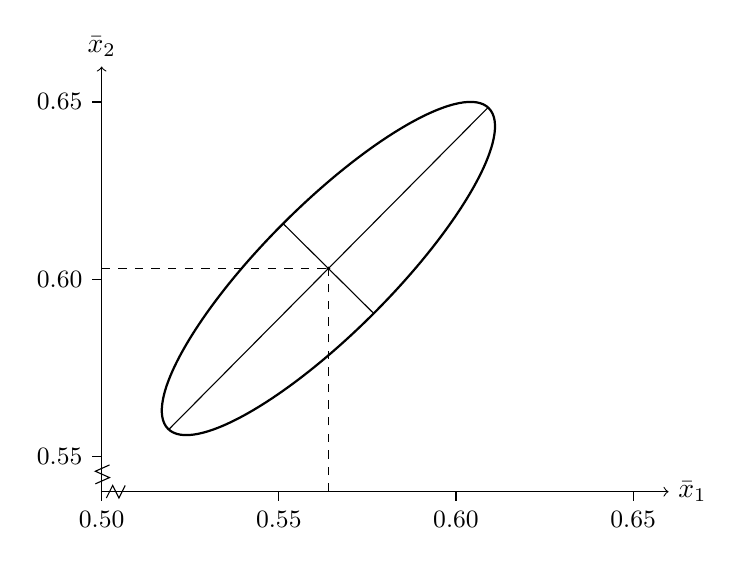
\begin{tikzpicture}[scale=1]
  \draw[->] (0,0) -- (7.2,0) node[right] {$\bar{x}_1$};
  \draw[->] (0,0) -- (0,5.4) node[above] {$\bar{x}_2$};
  \foreach \v/\p in {0.50/0,0.55/2.25,0.60/4.5,0.65/6.75}
    \draw (\p,0) -- (\p,-0.12) node[below] {\small $\v$};
  \foreach \v/\p in {0.55/0.45,0.60/2.70,0.65/4.95}
    \draw (0,\p) -- (-0.12,\p) node[left] {\small $\v$};
  % 坐标轴断裂记号
  \draw (0.30,0.08) -- (0.22,-0.08) -- (0.14,0.08) -- (0.06,-0.08);
  \draw (0.10,0.34) -- (-0.08,0.26) -- (0.10,0.18) -- (-0.08,0.10);
  % 中心虚线
  \draw[dashed] (2.88,0) -- (2.88,2.835);
  \draw[dashed] (0,2.835) -- (2.88,2.835);
  % 主、次轴
  \draw[thin] (0.852,0.790) -- (4.908,4.880);
  \draw[thin] (2.305,3.405) -- (3.455,2.265);
  % 置信椭圆
  \draw[thick,rotate around={45:(2.88,2.835)}] (2.88,2.835) ellipse (2.88cm and 0.81cm);
  \fill (2.88,2.835) circle (0.7pt);
\end{tikzpicture}
\phantomsection\label{fig:5.1}\mvcap{图 5.1\quad 微波炉辐射数据 $\boldsymbol{\mu}$ 的 95\% 置信椭圆}
\end{mvfigure}
